\chapter{The determinant that controls the approximants}
\label{cb_ch_wronskian}

The recurrence produces two rational sequences. Its most useful internal
certificate is the determinant of two adjacent coefficient pairs. This
determinant can be evaluated without knowing Catalan's constant, without a
decimal approximation to it, and without any assumption about its arithmetic
nature. It proves that the two sequences remain independent and gives an
exact description of the movement of their quotient.

\section{A determinant with a closed formula}

Write the recurrence in the form
\begin{equation}\label{cb_eq_rec_short}
 a_n w_{n+1}=q(n)w_n+c_nw_{n-1},\qquad n\geq1,
\end{equation}
where, in this chapter only,
\[
 a_n=(2n+1)^2(2n+2)^2p(n),\qquad
 c_n=(2n-1)^2(2n)^2p(n+1).
\]
These are recurrence coefficients, not the integer coefficients of a cleared
linear form used later. In particular, both are positive. The initial data are
\[
 u_0=1,\quad u_1=\frac74,\qquad
 v_0=0,\quad v_1=\frac{13}{8}.
\]
The polynomial $p(n)=20n^2-8n+1$ is positive for integer $n\geq0$.
Define the discrete Wronskian
\begin{equation}\label{cb_eq_W_def}
 W_n=u_{n+1}v_n-u_nv_{n+1},\qquad n\geq0.
\end{equation}
This convention fixes its sign. Reversing the two terms reverses every sign
in the subsequent formulas.

\begin{theorem}[Exact Wronskian]\label{cb_thm_W}
For every integer $n\geq0$,
\begin{equation}\label{cb_eq_W_closed}
 W_n=\frac{(-1)^{n+1}p(n+1)}{2(2n+1)^2(2n+2)^2}.
\end{equation}
In particular, $W_n\ne0$.
\end{theorem}

\begin{proof}
At $n=0$ the determinant is $-13/8$, which agrees with the displayed
formula because $p(1)=13$. For $n\geq1$, insert
\eqref{cb_eq_rec_short} into both terms of \eqref{cb_eq_W_def}. The terms
containing $q(n)u_nv_n$ cancel, leaving
\[
 W_n=\frac{c_n}{a_n}(u_{n-1}v_n-u_nv_{n-1})
     =-\frac{c_n}{a_n}W_{n-1}.
\]
Iterating this equality gives
\[
 W_n=(-1)^nW_0
 \prod_{j=1}^n
 \frac{(2j-1)^2(2j)^2p(j+1)}{(2j+1)^2(2j+2)^2p(j)}.
\]
There are two independent telescopes. The polynomial factors leave
$p(n+1)/p(1)$. The integer factors leave
$4/((2n+1)^2(2n+2)^2)$. Substituting $W_0=-13/8$ and $p(1)=13$
proves the identity. The empty product gives the same calculation at $n=0$.
\end{proof}

The proof is universal. A rational arithmetic check of its first 201
instances is an implementation check, not its logical foundation. The finite
check is still useful because it can detect a shifted index or a reversed
determinant convention. The first values make those conventions visible.

\begin{center}
\begin{tabular}{@{}rrrrr@{}}
\toprule
$n$ & $0$ & $1$ & $2$ & $3$\\
\midrule
$W_n$ & $-13/8$ & $65/288$ & $-157/1800$ & $289/6272$\\
\bottomrule
\end{tabular}
\end{center}

\begin{figure}[tbp]
\centering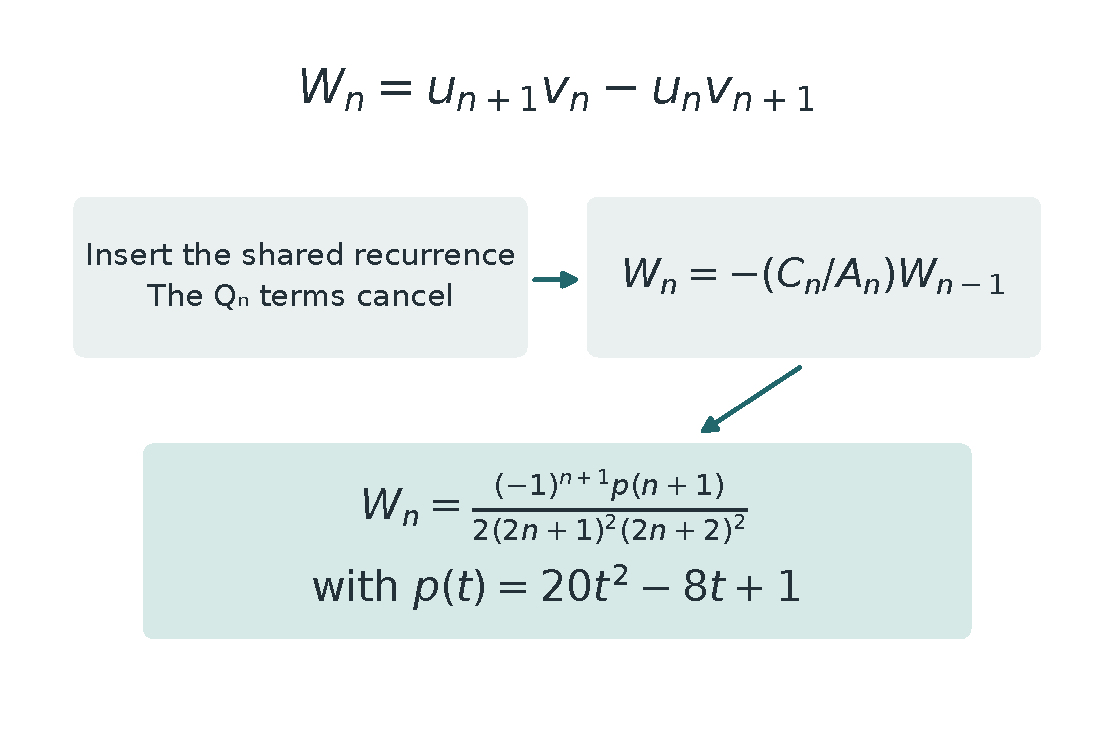
\includegraphics[width=0.92\linewidth]{../visual/figures/14_wronskian_identity.pdf}
\caption{The determinant recurrence loses the middle coefficient. Its
remaining product telescopes exactly. The figure illustrates the written
identity, which holds at every index.}\label{cb_fig_W_identity}
\end{figure}

\section{Positive coefficients and decreasing steps}

The next argument needs the positivity of $u_n$. It also needs a modest lower
bound on it, rather than a full asymptotic theorem. Both follow from the
recurrence. To see the relevant sign without relying on a plot, put $t=n-1$.
Direct polynomial expansion gives
\begin{align*}
 q(n)-a_n={}&3200t^6+24000t^5+73392t^4+117072t^3\\
            &+102768t^2+47112t+8827.
\end{align*}
Thus $q(n)>a_n>0$ for every $n\geq1$. Starting from $u_1>u_0>0$, the
recurrence implies
\[
 u_{n+1}>\frac{q(n)}{a_n}u_n>u_n.
\]
In particular $u_n\geq1$. This elementary bound is enough for the convergence
argument below.

Set
\begin{equation}\label{cb_eq_ratio_steps}
 r_n=\frac{v_n}{u_n},\qquad
 d_n=\frac{p(n+1)}{2(2n+1)^2(2n+2)^2u_nu_{n+1}}.
\end{equation}
The symbol $d_n$ denotes a positive rational step size. It is unrelated to
the least common multiples $L_N$ used in denominator clearing. Dividing the
Wronskian identity by $u_nu_{n+1}$ yields
\begin{equation}\label{cb_eq_alternating_steps}
 r_{n+1}-r_n=(-1)^n d_n.
\end{equation}
The movement of the approximants therefore alternates exactly.

\begin{lemma}[Strict decrease of the step sizes]\label{cb_lem_d_decrease}
The rational numbers $d_n$ are strictly positive, decrease strictly, and tend
to zero.
\end{lemma}

\begin{proof}
Positivity is immediate. For $n\geq1$, the determinant recurrence gives
\[
 \frac{d_n}{d_{n-1}}
 =\frac{c_n}{a_n}\frac{u_{n-1}}{u_{n+1}}<1.
\]
The strict inequality follows from
$a_nu_{n+1}=q(n)u_n+c_nu_{n-1}>c_nu_{n-1}$.
Finally $u_nu_{n+1}\geq1$, so
\[
 0<d_n\leq
 \frac{p(n+1)}{2(2n+1)^2(2n+2)^2}\longrightarrow0.
\]
No limiting characteristic root is needed for this conclusion.
\end{proof}

This is a useful example of the distinction between two arguments with
different jobs. The exponential rates from Zudilin's theorem describe the
quality of large approximants. The simple inequalities above establish
convergence and strict brackets directly from rational recurrence data.

\section{The limit and its exact rational brackets}

\begin{theorem}[Alternating brackets]\label{cb_thm_brackets}
There is a real number $L$ such that $r_n\to L$. For every $k\geq0$,
\begin{equation}\label{cb_eq_bracket}
 r_{2k}<L<r_{2k+1}.
\end{equation}
The even subsequence increases strictly and the odd subsequence decreases
strictly. For every $n\geq0$,
\begin{equation}\label{cb_eq_error_bounds}
 d_n-d_{n+1}<|L-r_n|<d_n,
 \qquad \operatorname{sign}(L-r_n)=(-1)^n.
\end{equation}
\end{theorem}

\begin{proof}
Equation \eqref{cb_eq_alternating_steps} and the preceding lemma identify
$r_n$ with partial sums of a convergent alternating series:
\[
 r_n=\sum_{j=0}^{n-1}(-1)^j d_j,
 \qquad L=\sum_{j=0}^{\infty}(-1)^j d_j.
\]
For the even subsequence,
$r_{2k+2}-r_{2k}=d_{2k}-d_{2k+1}>0$.
For the odd subsequence,
$r_{2k+3}-r_{2k+1}=-d_{2k+1}+d_{2k+2}<0$.
Their adjacent separation $d_{2k}$ tends to zero, so they have the same limit.
Strictness of both subsequences places that limit strictly between every
displayed pair. The alternating tail beginning with $d_n$ gives the sign
and upper bound in \eqref{cb_eq_error_bounds}. Pairing its first two terms
and then successive pairs gives the strict lower bound. All omitted pairs
are positive after multiplication by $(-1)^n$.
\end{proof}

The endpoints in \eqref{cb_eq_bracket} are exact rationals. For example,
the first few approximants are
\begin{center}
\begin{tabular}{@{}rl@{}}
\toprule
$n$ & $r_n$\\
\midrule
$0$ & $0$\\
$1$ & $13/14$\\
$2$ & $10699/11682$\\
$3$ & $8025653/8761950$\\
\bottomrule
\end{tabular}
\end{center}
There is no rounding decision in these brackets. Increasing the index
nests a narrower interval inside the earlier one. A program can use the
same determinant to check the interval width exactly.

The recurrence and its initial values establish a limit $L$. The statement
that this limit is $G$ is a separate mathematical identification. We use
Zudilin's Theorem 1 for that identification, with the normalization recorded
in source contract LC01 \cite{Zudilin2003}. After this external input,
\eqref{cb_eq_bracket} and \eqref{cb_eq_error_bounds} become exact bounds for
Catalan's constant and its rational approximants. In particular,
\begin{equation}\label{cb_eq_linear_error_sign}
 (-1)^n(u_nG-v_n)>0\qquad(n\geq0).
\end{equation}

This order of reasoning prevents a circular shortcut. Decimal agreement
between $r_n$ and a familiar constant does not identify a limit. Nor does
the nonzero Wronskian alone exclude equality between one particular
approximant and an arbitrary real number. The strict brackets supply
nonvanishing for the recurrence limit, and the source theorem then identifies
that limit with $G$.

\section{What this certificate does and does not settle}

The determinant settles several questions completely. Adjacent coefficient
pairs never become proportional. The ratio has a unique limit. Its even and
odd approximants bracket that limit, and their signs of error are fixed.
Each of these conclusions has a written argument valid at every index.

The determinant does not classify the limit as rational or irrational. A
sequence of distinct rational numbers with alternating errors can converge
to a rational number. Irrationality requires an additional comparison
between error size and the integer lattice after clearing denominators.
The Wronskian contributes exact nonvanishing and useful quantitative bounds,
but it does not pay the arithmetic cost of that clearing. The next chapters
keep these two requirements visible in the same coefficient construction.

\chapter{Integer coefficients and the corrected integral}
\label{cb_ch_integrality}

The rational recurrence is an efficient way to construct coefficients. It
does not by itself explain their denominators. A second description, in
terms of half integer binomial coefficients, gives a short universal
integrality proof. A third description, as a positive integral, supplies the
analytic error. Matching these descriptions requires care with constants.
In the source used here, one printed integral factor fails even at the
initial index. We record that failure and derive the factor used throughout
this edition.

\section{A coefficient identity, rather than an irrationality assumption}

Krattenthaler and Rivoal use coefficients $a_n,b_n$ for a linear form in
Catalan's constant \cite{KR2008}. These letters belong to their source and
do not denote the recurrence coefficients of the previous chapter. In the
normalization of this book their coefficients satisfy
\begin{equation}\label{cb_eq_KR_dictionary}
 a_n=-4u_n,\qquad b_n=-4v_n.
\end{equation}
The notation bridge is recorded in source contract LC05. After shifting the
source summation variable by one, their hypergeometric series is $-1/2$
times Zudilin's series. The source partial fraction expansion identifies
the two rational coefficients separately, giving
\eqref{cb_eq_KR_dictionary}.

It would be invalid to obtain this dictionary merely by equating two real
expressions in $G$ and then treating $1$ and $G$ as linearly independent over
$\Q$. That independence is exactly the irrationality under investigation.
Instead, take a formal variable $X$. The partial fraction coefficient
calculation identifies the polynomial $a_nX-b_n$ with
$-4(u_nX-v_n)$ in $\Q[X]$. Equality of coefficients in a polynomial ring
does not depend on the arithmetic nature of any later substitution for
$X$. This distinction also applies to the packet coefficients below.

The same source gives the explicit finite sum
\begin{equation}\label{cb_eq_halfbinomial}
 u_n=\sum_{j=0}^n
 \binom nj\binom{n-\tfrac12}{j}\binom{n+j-\tfrac12}{j},\qquad n\geq0.
\end{equation}
Here
\[
 \binom{x}{0}=1,\qquad
 \binom{x}{j}=\frac{x(x-1)\cdots(x-j+1)}{j!}\quad(j\geq1)
\]
defines the generalized binomial coefficient. Formula
\eqref{cb_eq_halfbinomial} is Lemma 3, equation (3.1), after the coefficient
normalization above. Its identification with the recurrence is an external
source input. The denominator argument that follows is elementary and is
written in full.

\section{The exact integer sequence}

Define
\begin{equation}\label{cb_eq_T_def}
 T_n=16^nu_n.
\end{equation}
The importance of the power $16^n$ is that it clears each summand of
\eqref{cb_eq_halfbinomial}, rather than relying on cancellation between
different summands.

\begin{lemma}[Half binomial denominators]\label{cb_lem_half_denom}
For integers $h,j\geq0$, the number
$4^j\binom{h-\tfrac12}{j}$ is an integer.
\end{lemma}

\begin{proof}
Work with formal power series, so no convergence issue arises. The central
binomial expansion gives
\[
 (1+4z)^{-1/2}=\sum_{k\geq0}(-1)^k\binom{2k}{k}z^k.
\]
Every coefficient is an integer. Multiplying by the integer polynomial
$(1+4z)^h$ preserves this property. The coefficient of $z^j$ in the product
is $4^j\binom{h-\tfrac12}{j}$. More explicitly it is
\[
 \sum_{\ell=0}^{\min(h,j)}
 \binom h\ell 4^\ell(-1)^{j-\ell}
 \binom{2(j-\ell)}{j-\ell},
\]
an integer sum.
\end{proof}

\begin{theorem}[Universal integrality of $T_n$]\label{cb_thm_T_integer}
For every integer $n\geq0$, $T_n$ is a positive integer. In fact, after
multiplication by $16^n$, each summand in
\eqref{cb_eq_halfbinomial} is an integer.
\end{theorem}

\begin{proof}
For $0\leq j\leq n$, apply the preceding lemma with $h=n$ and $h=n+j$.
The scaled summand is
\[
 16^{n-j}\binom nj
 \left(4^j\binom{n-\tfrac12}{j}\right)
 \left(4^j\binom{n+j-\tfrac12}{j}\right).
\]
All four factors are integers. Summing proves integrality. Every original
summand is positive: the generalized binomial factors have only positive
factors in their defining products when $j\leq n$. The $j=0$ term is one,
including at $n=0$. Thus the sum is positive.
\end{proof}

For example, the $n=2$ sum is
\[
 u_2=1+\frac{15}{2}+\frac{105}{64}=\frac{649}{64}.
\]
Multiplication by $16^2$ gives the three integers $256$, $1920$, and $420$,
whose sum is $T_2=2596$. This illustrates the proof at the level of individual
terms. The first sequence values are
\[
 T_0=1,\quad T_1=28,\quad T_2=2596,\quad
 T_3=311536,\quad T_4=41759524.
\]

The source theorem $16^na_n\in\Z$, combined with
\eqref{cb_eq_KR_dictionary}, would establish only $4T_n\in\Z$ directly.
Division by four is not an integrality argument. The half binomial proof
above establishes the stronger statement actually needed by the integer
packet construction. It removes a possible hidden dependence on a finite
exact division experiment.

The recurrence for $T_n$ is obtained by multiplying the original recurrence
by $16^{n+1}$:
\begin{equation}\label{cb_eq_T_recurrence}
 a_nT_{n+1}=16q(n)T_n+256c_nT_{n-1}\qquad(n\geq1).
\end{equation}
A program can therefore generate $T_n$ using integer numerators and exact
division by $a_n$. A nonzero remainder is a failed implementation check and
must terminate the computation. The written theorem establishes why exact
division succeeds universally for the correctly normalized recurrence.

\begin{figure}[tbp]
\centering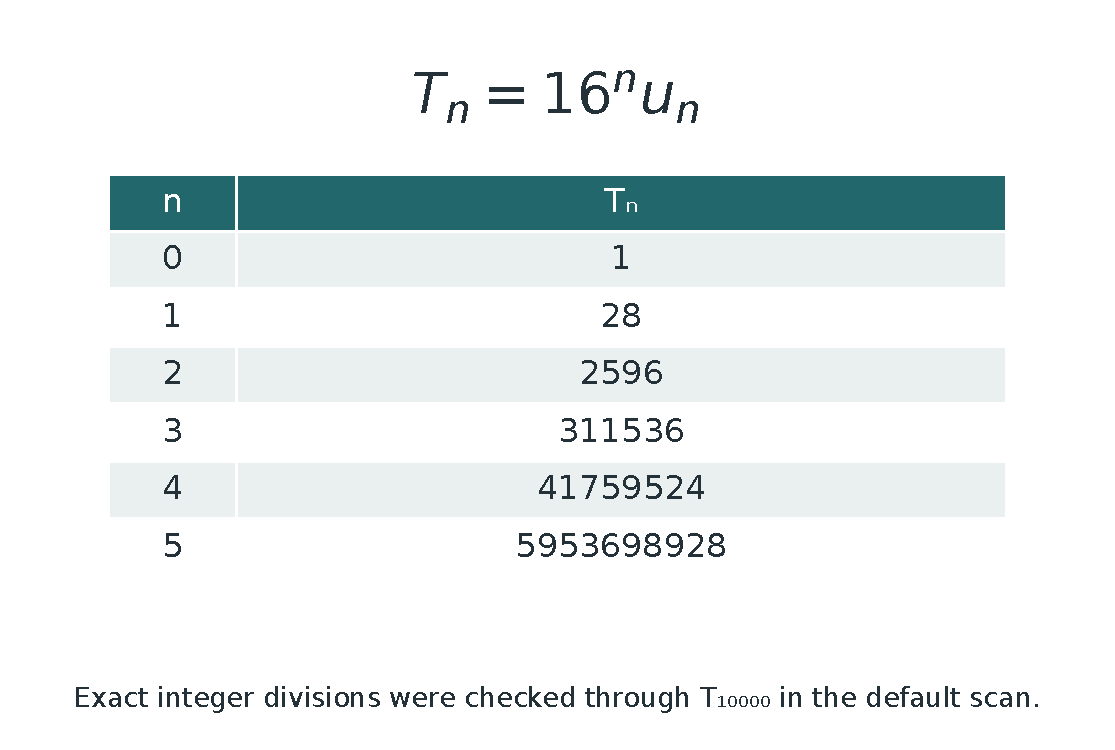
\includegraphics[width=0.93\linewidth]{../visual/figures/15_scaled_coefficients.pdf}
\caption{The recurrence coefficients become an integer sequence after
scaling by $16^n$. The finite values shown here accompany a universal
half binomial denominator proof.}\label{cb_fig_T}
\end{figure}

\section{The rational coefficient has a different clearing cost}

Put
\[
 L_N=\operatorname{lcm}(1,2,\ldots,N),\qquad L_0=1.
\]
The source's least common multiple notation is translated to $L_N$ here.
The letter $D$ will later denote an actual reduced denominator, which can
be much smaller than this universal clearing bound.
Krattenthaler and Rivoal's Theorem 2 gives
$16^nL_{2n}^2b_n\in\Z$ for positive integer $n$
\cite{KR2008}. In the present normalization it implies
\begin{equation}\label{cb_eq_v_sharp_clear}
 4\cdot16^nL_{2n}^2v_n\in\Z\qquad(n\geq0).
\end{equation}
The case $n=0$ is immediate from $v_0=0$. In particular the historical
script's weaker clearing factor, with $8$ in place of $4$, is valid at every
index. This is a source theorem about the rational coefficient. The
half binomial argument for $u_n$ does not automatically prove it.

Earlier asymptotic denominator bounds in Zudilin's remarks establish the
appropriate exponential scale with a logarithmic correction in the exponent
\cite{Zudilin2002}. They serve a different purpose from exact clearing at
every index. An asymptotic expression involving $o(n)$ should not be read
as a precise power of two that can be inserted into a finite computation.
For the packet arithmetic we use \eqref{cb_eq_v_sharp_clear} and the exact
integer theorem for $T_n$.

The finite direct product check in this release compares
\eqref{cb_eq_halfbinomial} with a separately indexed rational recurrence for
every $n=0,\ldots,50$. It checks 1326 summands, including the two half
binomial denominator statements and scaled integrality of each term. The
independent recurrence check extends through $n=500$ and verifies the weaker
factor $8$ clearing there. These are useful finite corroborations. The
external identity and the two universal arithmetic arguments have their
own evidence and remain distinct from those checks.

\section{A printed factor that fails at the initial index}

Consider the positive double integral
\begin{equation}\label{cb_eq_J_def}
 J_n=\int_0^1\!\int_0^1
 \frac{x^{n-1/2}(1-x)^ny^n(1-y)^{n-1/2}}
 {(1-xy)^{n+1}}\,\dd x\,\dd y,
 \qquad n\geq0.
\end{equation}
Zudilin's Theorem 3 prints $u_nG-v_n=(-1)^nJ_n/4$ in both the authenticated
arXiv version and the published journal PDF \cite{Zudilin2003}. With
$u_0=1$ and $v_0=0$, this would force $J_0=4G$.
The integral itself gives $J_0=8G$. Thus that printed factor cannot be used
with these initial conditions. This edition uses
\begin{equation}\label{cb_eq_J_correct}
 J_n=8(-1)^n(u_nG-v_n).
\end{equation}
No erratum was recovered in the bounded source search. The correction is
supported by the explicit derivation below, rather than an assertion that
a published correction exists.

The initial integral supplies a short diagnostic. Substitute $x=t^2$ and
$y=1-s^2$. Then
\begin{align*}
 J_0
 &=4\int_0^1\!\int_0^1\frac{\dd s\,\dd t}{1-t^2+t^2s^2}\\
 &=4\int_0^1\frac{\arcsin t}{t\sqrt{1-t^2}}\,\dd t
  =4\int_0^{\pi/2}\theta\csc\theta\,\dd\theta.
\end{align*}
Since an antiderivative of $\csc\theta$ is $\log\tan(\theta/2)$, integration
by parts yields
\[
 J_0=-4\int_0^{\pi/2}\log\tan(\theta/2)\,\dd\theta
     =-8\int_0^{\pi/4}\log\tan z\,\dd z=8G.
\]
Both boundary terms vanish. At zero this uses
$\theta\log\tan(\theta/2)\to0$, and at $\pi/2$ the logarithm is zero.

Checking one index detects the wrong normalization. It does not by itself
prove \eqref{cb_eq_J_correct} for every $n$. The next calculation explains
the all index extension and identifies its external transformation input.

\section{The all index normalization}

Expanding $(1-xy)^{-n-1}$ as its nonnegative binomial series and applying
Tonelli's theorem gives
\begin{equation}\label{cb_eq_beta_H}
 J_n=C_nH_n,
\end{equation}
where
\[
 C_n=\frac{\Gamma(n+1)^2\Gamma(n+\tfrac12)^2}
 {\Gamma(2n+\tfrac32)^2},
\]
and
\[
 H_n={}_3F_2\!\left(
 \begin{matrix}n+1,n+\tfrac12,n+1\\
 2n+\tfrac32,2n+\tfrac32\end{matrix};1\right).
\]
Indeed, the two beta integrals in the term with index $k$ are
$B(n+\tfrac12+k,n+1)$ and $B(n+1+k,n+\tfrac12)$.
Their ratios to the corresponding $k=0$ integrals give exactly the displayed
hypergeometric parameters. The excess of the lower parameters over the
upper parameters is $n+1/2>0$, so the series converges for every $n\geq0$.

Let $E_n$ denote the well poised ${}_6F_5$ series at $-1$ in Zudilin's
displayed Whipple transformation, with
$a=3n+1$, $b=c=d=n+1/2$, and $e=n+1$. The transformation states
\[
 H_n=\frac{\Gamma(3n+2)\Gamma(n+\tfrac12)}
 {\Gamma(2n+\tfrac32)\Gamma(2n+1)}E_n.
\]
Its condition $\operatorname{Re}(1+a-d-e)>0$ becomes $n+1/2>0$ here.
The displayed prefactor of the source hypergeometric form $F_n^{\rm src}$
is
\[
 F_n^{\rm src}=(-1)^n
 \frac{\Gamma(n+1)^2\Gamma(3n+2)\Gamma(n+\tfrac12)^3}
 {\Gamma(2n+\tfrac32)^3\Gamma(2n+1)}E_n.
\]
Substitution in \eqref{cb_eq_beta_H} therefore gives
$F_n^{\rm src}=(-1)^nJ_n$. There is no additional factor two in the gamma
cancellation. The formal partial fraction coefficient identification in
the same source gives $F_n^{\rm src}=8(u_nG-v_n)$, with the recurrence
initial data used here. Combining these two identities proves
\eqref{cb_eq_J_correct} at every index.

The beta integral expansion and prefactor cancellation are written
calculations. The Whipple transformation and the partial fraction
identification are external mathematical inputs from the authenticated
paper. Their precise roles are recorded in LC03 and the accompanying
normalization audit. The independent initial integral agrees with the
result, and Eskandari's coefficient normalization uses the same factor $8$
\cite{Eskandari2026}.

\section{Three descriptions, three different guarantees}

The recurrence permits efficient exact computation. The half binomial
formula proves that $16^nu_n$ is always an integer. The integral describes
the error and makes its sign transparent after the corrected normalization.
These descriptions agree, but each answers a different question. Keeping
their roles distinct prevents a finite arithmetic check from being mistaken
for an analytic theorem, or a positive integral from being mistaken for
denominator control. The packet construction will use all three.

\chapter{The binomial packet and the integral filter}
\label{cb_ch_packets}

The packet combines a finite block of recurrence coefficients. Its integer
part is a positive binomial sum, while its error part is a signed integral.
These two facts coexist because the signs in the original error already
alternate. The packet removes those coefficient signs and replaces them
with a polynomial filter inside the integral. That filter is useful for
approximation, but its changing sign imposes a real restriction on any
nonvanishing argument.

\section{A finite transform with an exact additive evolution}

For integers $n,m\geq0$, define
\begin{align}
 S_{n,m}&=\sum_{i=0}^m\binom miT_{n+i},\label{cb_eq_S_def}\\
 H_{n,m}&=\sum_{i=0}^m\binom mi16^{n+i}v_{n+i}.
 \label{cb_eq_H_packet_def}
\end{align}
The two index symbol $H_{n,m}$ denotes a rational packet coefficient. It is
distinct from the hypergeometric function $H_n$ used in the integral
normalization derivation. The theorem on $T_n$ proves
$S_{n,m}\in\Z_{>0}$ at every pair. The coefficient $H_{n,m}$ is rational
and requires separate denominator clearing.

\begin{proposition}[Pascal evolution]\label{cb_prop_Pascal}
For $n,m\geq0$,
\begin{equation}\label{cb_eq_Pascal}
 S_{n,m+1}=S_{n,m}+S_{n+1,m}.
\end{equation}
The same identity holds with $H$ in place of $S$.
\end{proposition}

\begin{proof}
Use $\binom{m+1}{i}=\binom mi+\binom m{i-1}$, with out of range binomial
coefficients interpreted as zero. The first contribution is $S_{n,m}$.
Changing $i$ to $i+1$ in the second contribution gives $S_{n+1,m}$. The
argument uses only the finite weights, so it applies to either seed
sequence.
\end{proof}

At $m=0$, the packet is just $S_{n,0}=T_n$. The first two nontrivial rows
are
\[
 S_{n,1}=T_n+T_{n+1},\qquad
 S_{n,2}=T_n+2T_{n+1}+T_{n+2}.
\]
For example $S_{1,1}=28+2596=2624$. The Pascal identity produces exactly
the same integer as direct evaluation of its defining sum. This agreement
between an additive row evolution and a direct weighted sum gives two
different implementations of the finite transform.

If $E$ denotes the shift operator $(Ef)_n=f_{n+1}$, the packet is
$(1+E)^mT$ at index $n$. This is an identity about a finite polynomial in
one shift. It does not introduce a further assumption about recurrence
solutions or convergence. Reduction modulo a power of two commutes with
this polynomial, which is the basis of the valuation computation in the
next chapter.

\begin{figure}[tbp]
\centering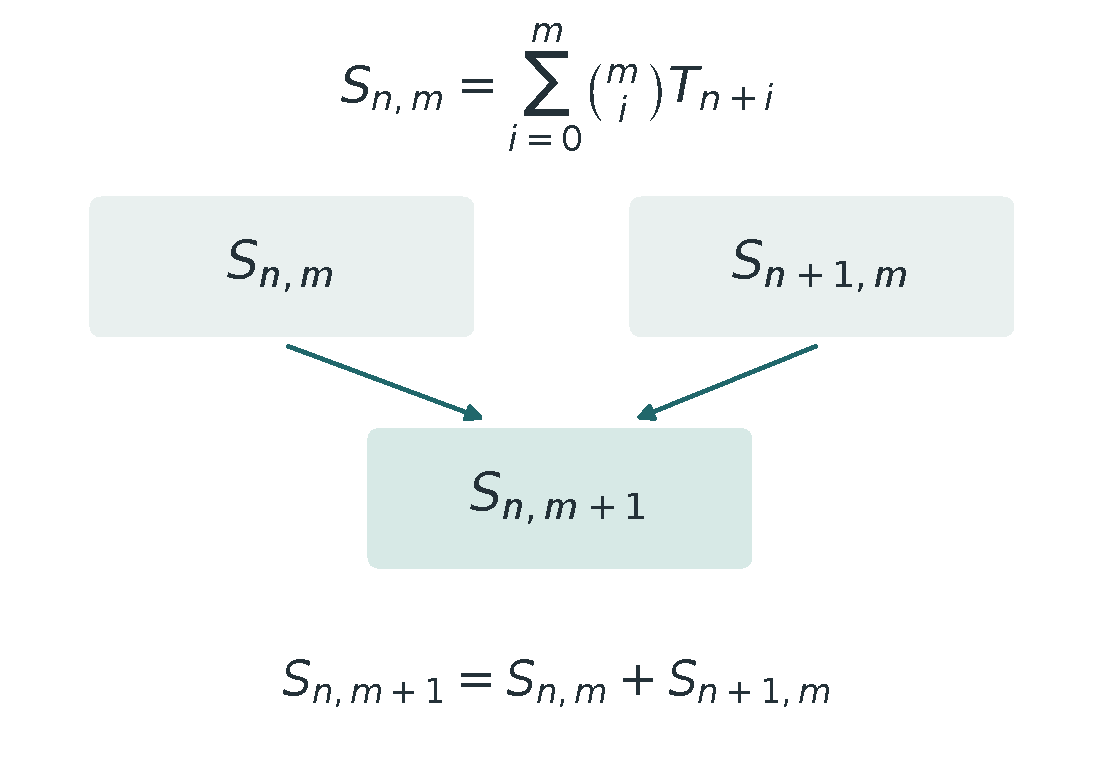
\includegraphics[width=0.91\linewidth]{../visual/figures/16_pascal_transform.pdf}
\caption{Each new packet row is the sum of adjacent entries in the
preceding row. This exact identity is also valid after modular reduction.}
\label{cb_fig_Pascal}
\end{figure}

\section{The source filter and the raw form}

Eskandari's preprint applies the filter
\begin{equation}\label{cb_eq_Jtilde}
 \widetilde J_{n,m}=\sum_{i=0}^m(-16)^i\binom miJ_{n+i}
 \qquad(n,m\geq0)
\end{equation}
to the integral family \cite{Eskandari2026}. The filter and its approximation
analysis are external work. This book examines its coefficient arithmetic
and the finite evidence recovered from the project's script.

Substitute the corrected normalization
$J_k=8(-1)^k(u_kG-v_k)$ into \eqref{cb_eq_Jtilde}. The two factors
$(-1)^i$ cancel. Thus
\begin{equation}\label{cb_eq_Jtilde_coeffs}
 \widetilde J_{n,m}=8(-1)^n16^{-n}(S_{n,m}G-H_{n,m}).
\end{equation}
Define the raw packet form
\begin{equation}\label{cb_eq_raw_F}
 F_{n,m}=16^n\widetilde J_{n,m}
        =8(-1)^n(S_{n,m}G-H_{n,m}).
\end{equation}
The adjective raw means that the common denominator of $H_{n,m}$ has not
yet been cleared. It does not mean that $F_{n,m}$ is an integer linear form.
The coefficient of $G$ is an integer, but the other coefficient may be
rational.

This normalization is important for comparison with historical data.
Multiplying or dividing a linear form by a growing power changes its
displayed decay rate. The integral filter is $\widetilde J_{n,m}$, while
the recorded arithmetic form $F_{n,m}$ is $16^n$ times it. Their signs and
zeros agree because $16^n>0$. Their logarithmic size per unit $n$ differs by
$\log16$.

\section{The measure and its sign changing polynomial}

On the open unit square, set
\begin{equation}\label{cb_eq_psi_mu}
 \psi(x,y)=\frac{xy(1-x)(1-y)}{1-xy},\qquad
 \dd\mu=\frac{\dd x\,\dd y}{\sqrt{x(1-y)}(1-xy)}.
\end{equation}
The factor $1-xy$ is outside the square root. Moving that factor inside, as in
\[
 \frac{\dd x\,\dd y}{\sqrt{x(1-y)(1-xy)}},
\]
would represent a different integral. With the measure in \eqref{cb_eq_psi_mu},
\[
 J_n=\int_{(0,1)^2}\psi^n\,\dd\mu,
 \qquad
 \widetilde J_{n,m}=\int_{(0,1)^2}\psi^n(1-16\psi)^m\,\dd\mu.
\]
The second identity follows by the ordinary binomial theorem inside a
finite sum. The total measure is $J_0=8G<\infty$.

The kernel has a simple maximum that also explains why the filter changes
sign. Put $r=\sqrt{xy}$. Since $x+y\geq2r$,
\[
 \psi(x,y)\leq\frac{r^2(1-r)^2}{1-r^2}
              =\frac{r^2(1-r)}{1+r},\qquad0<r<1.
\]
Equality is achieved when $x=y=r$. The derivative of the last expression
is
\[
 \frac{2r(1-r-r^2)}{(1+r)^2}.
\]
It has its interior maximum at $r=\phi^{-1}$, where
$\phi=(1+\sqrt5)/2$. Since $1-r=r^2$ there, the maximum is
\begin{equation}\label{cb_eq_psi_max}
 \max\psi=\phi^{-5}\approx0.09017.
\end{equation}
This is greater than $1/16$. One can already see a negative filter value
at $x=y=1/2$, where $\psi=1/12$ and $1-16\psi=-1/3$.
Near the sides of the square $\psi$ is small and the filter is positive.

\begin{theorem}[Nonvanishing for even filter order]\label{cb_thm_even_positive}
For every $n\geq0$ and every even integer $m\geq0$,
$\widetilde J_{n,m}>0$ and $F_{n,m}>0$.
\end{theorem}

\begin{proof}
For even $m$, the integrand $\psi^n(1-16\psi)^m$ is nonnegative. It is
strictly positive on an open subset of the square with $0<\psi<1/16$.
The measure has positive density there. Hence its integral is strictly
positive. It is finite because $\psi$ and $1-16\psi$ are bounded and
$\mu$ has finite total mass. Multiplication by $16^n$ preserves positivity.
\end{proof}

This theorem includes $m=0$ and $n=0$. It does not require that $G$ be
irrational. Indeed, positivity is one of the ingredients that an eventual
irrationality criterion would combine with sufficiently small cleared
integer forms. The even order restriction is easy to impose along an
asymptotic slope by choosing $m(n)$ to be the nearest suitable even integer.
The change in $m/n$ then tends to zero.

\section{The odd sign hypothesis failed}

For odd $m$, the polynomial factor changes sign, so the preceding positivity
proof does not apply. A proposed shortcut was the sign pattern
$\operatorname{sign}F_{n,m}=(-1)^m$. The finite audit falsified it. The first
counterexample is the pair $(n,m)=(1,1)$.

Using $u_1=7/4$, $v_1=13/8$, $u_2=649/64$ and $v_2=10699/1152$, one obtains
\[
 S_{1,1}=2624,\qquad H_{1,1}=\frac{21632}{9}.
\]
Consequently
\begin{equation}\label{cb_eq_odd_counterexample}
 F_{1,1}=\frac{173056}{9}-20992G>0.
\end{equation}
The inequality is certified by the exact rational enclosure of $G$ recorded
in the independent computation. The threshold for it is $G<338/369$.
The enclosure lies strictly below that rational number. Thus this form is
positive although $m$ is odd, contradicting the proposed pattern.
The sign is decided by rational interval endpoints, rather than floating
point subtraction between nearly equal numbers.

The audit checks 860 pairs with $1\leq n\leq20$ and $0\leq m\leq4n$.
Every tested form is certified nonzero, but a number of odd pairs violate
the proposed pattern. Both positive and negative odd order forms occur in
that finite domain. For example the recorded signs at $(1,1)$ and $(2,1)$
are opposite. These observations do not establish nonvanishing for every
odd pair. This edition retains the failed hypothesis and its diagnostic
record, and uses the universal even order theorem when nonvanishing is
needed in a global implication.

\begin{figure}[tbp]
\centering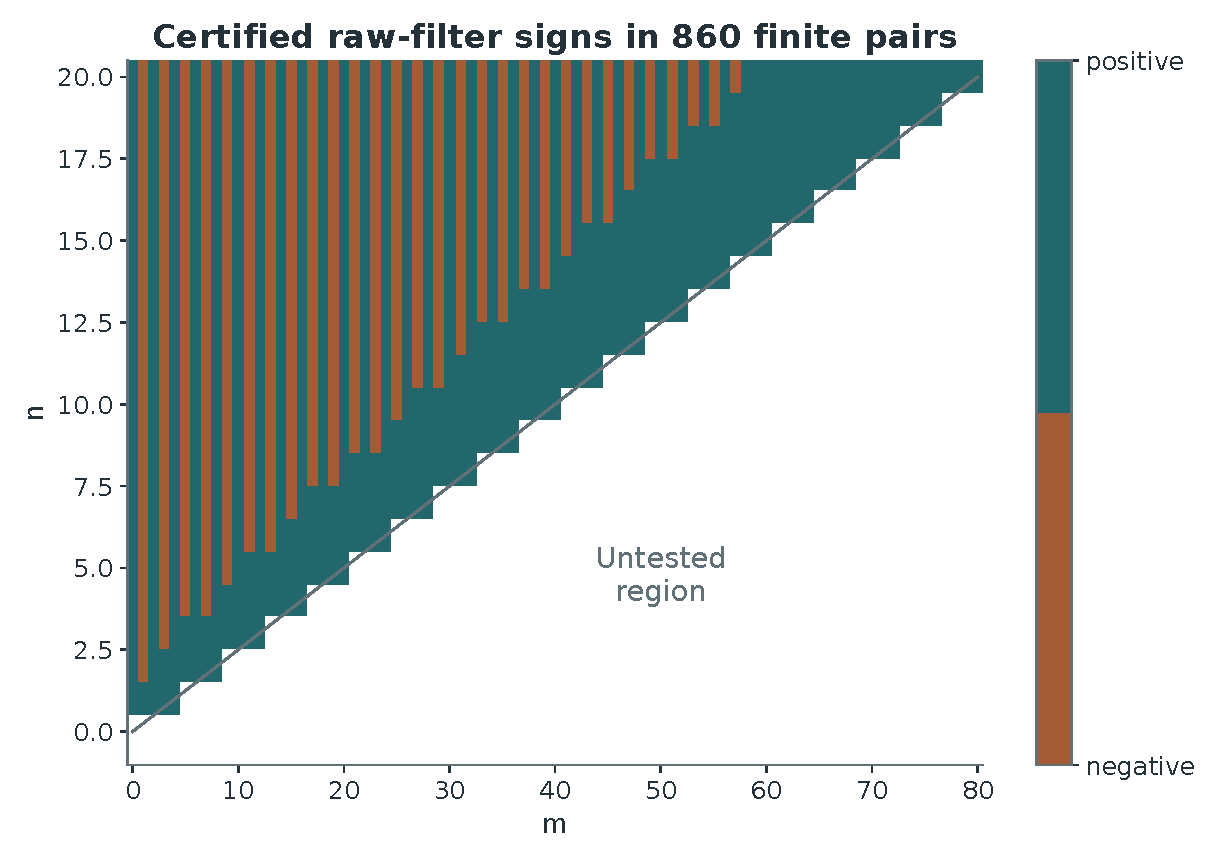
\includegraphics[width=0.91\linewidth]{../visual/figures/27_filter_signs.pdf}
\caption{Certified signs in a bounded packet domain. Even filter orders
have a universal positivity proof. Odd filter orders display both signs,
and the proposed alternating rule fails.}\label{cb_fig_filter_signs}
\end{figure}

\section{The exact historical integer pair}

Let $N=n+m$ and put
\begin{equation}\label{cb_eq_C_clear}
 C_{n,m}=L_{2N}^2.
\end{equation}
The pair produced by the historical script is
\begin{align}
 A_{n,m}&=8(-1)^nC_{n,m}S_{n,m},\label{cb_eq_historical_A}\\
 B_{n,m}&=8(-1)^nC_{n,m}H_{n,m}.
 \label{cb_eq_historical_B}
\end{align}
Both coefficients are integers. Integrality of $A$ follows from that of
$S$. For $B$, each index $k=n+i$ satisfies $k\leq N$, so $L_{2k}$ divides
$L_{2N}$. The sharp source clearing
$4\cdot16^kL_{2k}^2v_k\in\Z$ therefore proves integrality term by term
after multiplication by $8L_{2N}^2$. The binomial weights introduce no
further denominators.

The cleared linear form is exactly
\begin{equation}\label{cb_eq_cleared_integral}
 A_{n,m}G-B_{n,m}
 =C_{n,m}F_{n,m}
 =16^nL_{2N}^2\widetilde J_{n,m}.
\end{equation}
Every factor in this identity has a fixed meaning. In particular, the
historical pair includes the constant factor $8$ and uses the possibly
redundant common clearing $L_{2N}^2$. It is not automatically a primitive
integer pair. Dividing out its common content is a separate arithmetic
operation examined later.

At $m=0$ the construction reduces to the cleared original recurrence form.
At $n=0$ all identities remain valid with $T_0=1$, $v_0=0$, and $L_0=1$.
The large valuation scan starts at $n=1$ for its stated triangular domain,
but that computational choice does not restrict the algebraic identities
proved in this chapter.

\chapter{What the modular valuation scan proves}
\label{cb_ch_modular}

The packet coefficients grow rapidly, but their divisibility by two can be
decided from a sufficiently precise residue. The large scan uses that fact
to evaluate a finite domain efficiently. Its exactness comes from a simple
valuation lemma and from the absence of zero residues. Its limitation comes
from the finite domain. These are separate issues: modular arithmetic can
give an exact answer at millions of pairs without producing a theorem at
every pair.

\section{The residue lemma}

For a nonzero integer $z$, let $v_2(z)$ be the largest nonnegative integer
$t$ such that $2^t$ divides $z$. Thus $v_2(12)=2$ and $v_2(1)=0$.
The value $v_2(0)$ is infinite rather than a finite integer. Our packet
$S_{n,m}$ is strictly positive, so its valuation is always finite, even when
a finite precision residue is zero.

\begin{lemma}[Exactness below the precision ceiling]\label{cb_lem_mod_v2}
Let $K\geq1$, let $z\ne0$ be an integer, and let $\rho$ be its least
nonnegative residue modulo $2^K$. If $\rho\ne0$, then
\[
 v_2(z)=v_2(\rho)<K.
\]
If $\rho=0$, the residue gives only $v_2(z)\geq K$.
\end{lemma}

\begin{proof}
Write $z=\rho+2^Kh$. If $\rho=2^ta$ with $a$ odd and $t<K$, then
$z=2^t(a+2^{K-t}h)$ and the parenthesis is odd. Hence the valuation is
exactly $t$. If $\rho=0$, the congruence says that $2^K$ divides $z$, but
contains no information about further powers of two.
\end{proof}

For example, the residue of $S_{1,1}=2624$ modulo $2^{128}$ is nonzero and
has valuation six. Its residue modulo $16$ is zero, which says only that
its valuation is at least four. The integer itself did not change. The
precision changed the information available about it.

A program that returns a number $K$ for a zero residue must attach a lower
bound interpretation to that number. It must not use it as an exact
valuation or as an exact maximum of the domain. The historical script
counts unresolved residues and includes an explicit exactness flag. The
release tests that flag deliberately.

\begin{figure}[tbp]
\centering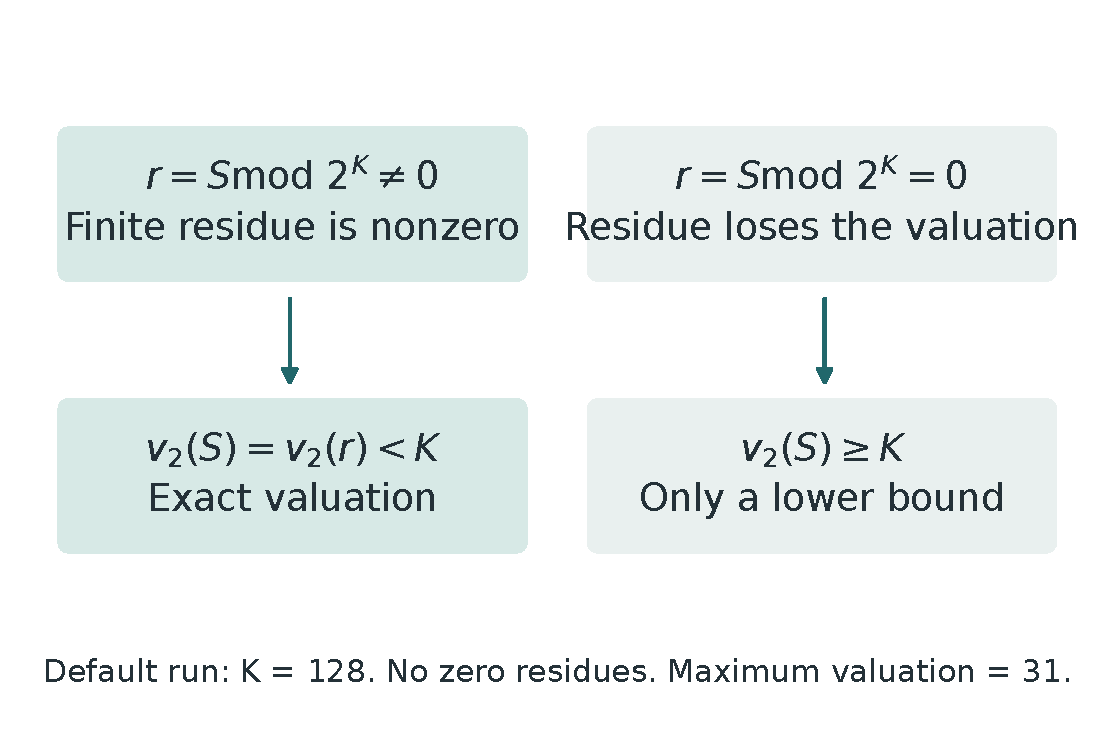
\includegraphics[width=0.91\linewidth]{../visual/figures/18_modular_exactness.pdf}
\caption{A nonzero residue modulo $2^K$ determines the exact valuation.
A zero residue reaches the precision ceiling and supplies only a lower
bound.}\label{cb_fig_mod_exactness}
\end{figure}

\section{The domain and the Pascal computation}

For a positive integer $N$, the scanned domain is
\begin{equation}\label{cb_eq_scan_domain}
 \mathcal D_N=\{(n,m):1\leq n\leq N,\ 0\leq m\leq4n\}.
\end{equation}
The number of scanned pairs is
\begin{equation}\label{cb_eq_scan_count}
 \sum_{n=1}^N(4n+1)=2N^2+3N.
\end{equation}
The upper slope $4$ is part of the experiment's definition. The
scan supplies no information about pairs above this boundary or with
$n>N$.

The computation first constructs $T_0,\ldots,T_{5N}$ through the exact
integer recurrence. It then reduces these integers modulo $2^K$. The
resulting array is the packet row with $m=0$. At each subsequent row,
Pascal evolution replaces adjacent entries by their sum modulo $2^K$.
Induction from \eqref{cb_eq_Pascal} proves that every entry read by the
scan is the exact residue of its packet sum.

For a fixed row $m$, the allowed indices are
\[
 \max(1,\lceil m/4\rceil)\leq n\leq N.
\]
Rows are needed through $m=4N$. In row $m$, the seed array is sufficient
for every $n\leq5N-m$. At the extreme row $m=4N$ this bound is exactly
$n\leq N$. Thus no scanned entry needs an unconstructed seed term.
The algorithm evaluates additional row entries to support later rows.
Those additions do not enlarge the declared set of scanned pairs.

This procedure uses full exact integers to construct the seed sequence,
including checks of all division remainders. Only the subsequent packet
row evolution is performed at fixed modular precision. Describing the
entire calculation as a floating point estimate would therefore be
incorrect. Describing its finite result as a uniform asymptotic theorem
would also be incorrect.

\section{The reproduced 2000 row result}

The historical run takes $N=2000$ and $K=128$. The release reran the
unchanged historical algorithm and compared its result with the recovered
output. The finite arithmetic results agree. In the domain
$\mathcal D_{2000}$ there are exactly $8{,}006{,}000$ pairs. Every observed
residue is nonzero, so the residue lemma applies at every pair. The exact
maximum valuation in this finite domain is
\begin{equation}\label{cb_eq_finite_max}
 \max_{(n,m)\in\mathcal D_{2000}}v_2(S_{n,m})=31.
\end{equation}
The recorded maximizing pair is $(1466,2113)$. The record reports the
first maximum encountered in its scan order and makes no assertion that
this maximizing pair is unique.

There is a generous precision margin: the largest observed valuation is
$31<128$, and there are zero unresolved residues. Consequently the finite
maximum is exact, rather than a maximum of truncated lower bounds. No
statistical confidence interval is involved. The essential qualification
is the finite domain in \eqref{cb_eq_finite_max}.

\begin{figure}[tbp]
\centering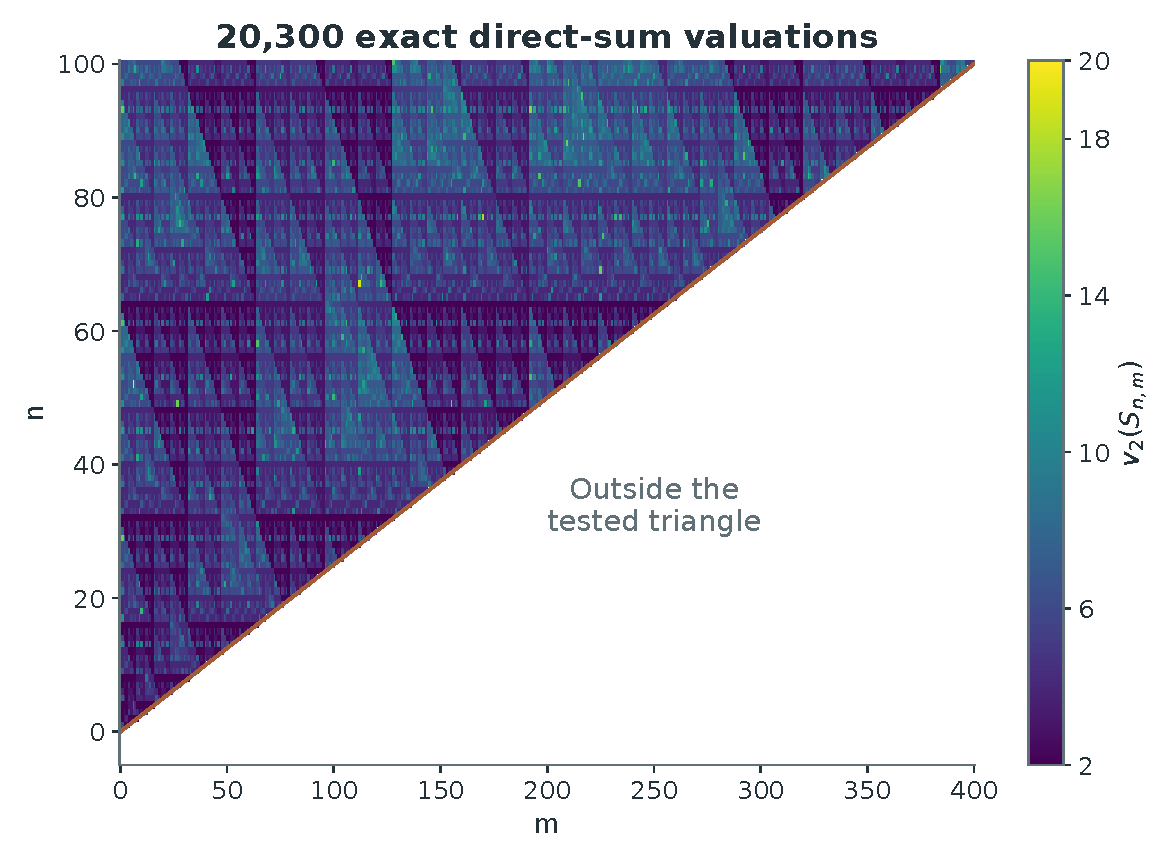
\includegraphics[width=0.93\linewidth]{../visual/figures/19_v2_heatmap.pdf}
\caption{An exact valuation grid in the smaller independently checked
domain. The pattern can suggest questions about cancellation, but its
appearance does not imply an asymptotic law.}\label{cb_fig_v2_grid}
\end{figure}

\section{A comparison at every pair and a full integer witness}

The historical smaller crosscheck reports the same maximum from direct
sums through $N=100$. Matching only two summary maxima would be a weak
comparison: different entry values can share the same maximum. The release
therefore compares every pair in $\mathcal D_{100}$.

For each of its $20{,}300$ pairs, a separate implementation evaluates
\[
 \sum_{i=0}^m\binom miT_{n+i}
\]
as a full positive integer and compares both its residue modulo $2^{128}$
and its exact valuation with the Pascal row entry. All pairs agree. There
are no zero residues. The finite maximum is $20$, recorded first at
$(52,6)$ in the direct comparison's order.

The direct summation and Pascal evolution use different operations on the
same seed data. This catches errors in the packet transform that agreement
between two copies of the same row update could miss. A separately indexed
rational recurrence also checks the seed construction through $n=500$.
These comparisons still share the intended recurrence formulas and require
the literature normalization contract. Their independence is operational,
not a claim that all common source risk has disappeared.

The pair $(1466,2113)$ was additionally evaluated as a full integer, along
with four neighboring pairs. The maximizing witness has bit length
$26{,}743$ and exact valuation $31$. Its complete hexadecimal integer is
included in the evidence bundle with a hash. The neighboring valuations
are much smaller:
\begin{center}
\begin{tabular}{@{}rrr@{}}
\toprule
$n$ & $m$ & $v_2(S_{n,m})$\\
\midrule
$1465$ & $2113$ & $12$\\
$1466$ & $2112$ & $13$\\
$1466$ & $2113$ & $31$\\
$1466$ & $2114$ & $11$\\
$1467$ & $2113$ & $11$\\
\bottomrule
\end{tabular}
\end{center}
These five full integer computations corroborate a particular spike.
They do not establish the maximum over millions of pairs. The exhaustive
modular scan with no unresolved residues establishes that finite maximum.

\section{A deliberate precision failure}

The release includes a diagnostic with $N=3$ and just $K=4$ bits of
precision. There are 27 pairs. Eight residues are zero, so those eight
valuations are unresolved at this precision. The historical scan records
a ceiling value of four and sets its exactness flag to false. Full integer
evaluation shows that the actual finite maximum is six.

This is a successful diagnostic of a deliberately insufficient precision,
not an exact four bit maximum. It demonstrates why the unresolved count
is load bearing. The program's numerical field alone would be misleading
if read without its flag. In the actual 128 bit release run, the same
classification logic reports zero unresolved entries and therefore
permits an exact interpretation.

One should also distinguish this diagnostic from the failed odd filter
sign hypothesis. The low precision test intentionally triggers a known
information limitation and verifies that it is reported correctly. The
odd sign test disproves a proposed mathematical pattern. The evidence
bundle records both, with their different meanings.

\section{Why a finite maximum does not settle growth}

The largest valuation seen so far is small compared with the largest
index. That observation motivates a question such as
\[
 v_2(S_{n,m})=o(n+m)
\]
along a specified family of packet indices. It does not prove the answer.
A universal statement needs quantified control beyond the scanned domain,
with the family of $m$ values and the meaning of uniformity stated
explicitly. A maximum found on a bounded grid cannot rule out later spikes
of a different scale.

Even a proved estimate for $v_2(S_{n,m})$ would address only one prime and
one coefficient. The common content of the full integer pair involves both
coefficients, their clearing factor, and odd prime divisibility. The scan
therefore supplies a precise finite arithmetic fact and a well defined
research question. It is not, by itself, the missing denominator theorem
or an irrationality proof.

The next stage should preserve this clarity. A proposed global valuation
bound must have a written argument valid at every permitted index. A
claimed content improvement must refer to the exact integer pair or to
its primitive reduction. A decay claim must include the clearing factors
that turn a real error into an integer linear form. The finite experiment
can guide those arguments and test their implementations, while the
global conclusion remains subject to its own proof.

